\documentclass[12pt]{article}

\usepackage{tcc-template}
\usepackage{graphicx,url}
\graphicspath{{figs/}}
\usepackage[utf8]{inputenc}
\usepackage[brazil]{babel}
% \usepackage[latin1]{inputenc}
\usepackage{amsmath}
\usepackage{listings}
\usepackage{xcolor} % Para cores (opcional, mas fica bonito)
\usepackage{tikz}
\usepackage{pgf-umlsd}   % Para diagramas de sequência UML
\usetikzlibrary{positioning, arrows.meta, calc}
\usepackage{pgfplots}
\usepackage[T1]{fontenc}
\pgfplotsset{compat=1.18}
\usepackage{booktabs}
\usepackage{siunitx}

% Configuração global do estilo de código
\lstset{
  language=Python,                 % Linguagem (Python, Java, JSON, etc.)
  basicstyle=\ttfamily\small,      % Fonte monoespaçada (Courier)
  breaklines=true,                 % Quebra linhas longas automaticamente
  frame=single,                    % Borda ao redor do código
  numbers=left,                    % Numeração das linhas à esquerda
  numberstyle=\tiny\color{gray},   % Estilo da numeração
  tabsize=2,                       % Tamanho da tabulação
  showstringspaces=false,          % Não mostra espaços sublinhados
  captionpos=b,                    % Legenda embaixo
  escapeinside={\%*}{*)},          % Permite LaTeX dentro do código (ex: equações)
}

\sloppy

\title{Wumpus Verse: Um Protótipo de Plataforma Web para Desenvolvimento e Avaliação de Agentes no Mundo de Wumpus}

\author{José R. M. Pereira\inst{1}, Williams D. E. Duarte\inst{2}, Pedro P. V. Barroso\inst{3}, Otávio N. Teixeira\inst{4}}


\address{Campus Universitário de Tucuruí (CAMTUC) \\ Universidade Federal do Pará (UFPA)\\ Tucuruí -- PA -- Brazil
\nextinstitute
  Núcleo de Desenvolvimento da Amazônia (NDAE) \\ Universidade Federal do Pará (UFPA)\\ Tucuruí -- PA -- Brazil
  \email{jose.r.maciel@outlook.com,\{pedrovbarroso087, onoura, davidduart04\}@gmail.com}
}

\begin{document} 

\maketitle

\begin{abstract}
  This paper presents the prototype of a web platform designed to provide an intuitive, pleasant, and practical testing environment for intelligent agents within the Wumpus World. Aimed at experimentation and research in Artificial Intelligence, the tool allows users to freely customize environments and configure different types of agents. The system enables the execution of combined experiments with performance metrics generation, while ensuring the persistence and reproduction of past simulations. The platform simplifies practical experimentation by providing a visual ecosystem that brings users closer to artificial intelligence concepts.
\end{abstract}
     
\begin{resumo} 
  Este trabalho apresenta o protótipo de uma plataforma web projetada para oferecer um ambiente de testes intuitivo, agradável e prático para agentes inteligentes no ambiente do Mundo do Wumpus. Voltada para a experimentação e à pesquisa em Inteligência Artificial, a ferramenta permite que o usuário customize ambientes livremente e configure diferentes tipos de agentes. O sistema viabiliza a execução de experimentos combinados com geração de métricas de desempenho, além de garantir a persistência e a reprodução de simulações passadas. A plataforma simplifica a experimentação prática, fornecendo um ecossistema visual que aproxima usuários de conceitos de inteligência artificial.
\end{resumo}

\section{Introdução} \label{sec:firstpage}

O ensino e a experimentação em Inteligência Artificial (IA) frequentemente utilizam ambientes simplificados que permitem explorar conceitos fundamentais sem a complexidade inerente aos problemas do mundo real. Nesse contexto, o Mundo do Wumpus destaca-se como um dos exemplos clássicos para o estudo de agentes inteligentes e processos de tomada de decisão, combinando regras relativamente simples com desafios relacionados à percepção parcial do ambiente, raciocínio sob incerteza e planejamento. O conceito tem origem no jogo Hunt the Wumpus, proposto por \cite{yob1975hunt}, com o objetivo de criar um desafio de exploração e sobrevivência em um ambiente desconhecido e dinâmico, envolvendo elementos como armadilhas, um inimigo oculto e a necessidade de localização espacial do jogador. Posteriormente, \cite{russell2021artificial} incorporaram esse cenário ao contexto da Inteligência Artificial, consolidando o Mundo do Wumpus como um ambiente clássico para o estudo de agentes inteligentes, representação do conhecimento e mecanismos de inferência lógica.

No Mundo do Wumpus, o agente navega em um grid parcialmente observável contendo poços, uma criatura hostil e ouro, devendo coletar o ouro e retornar à saída sem ser eliminado. O agente utiliza percepções locais (como brisa para indicar poços adjacentes e fedor par proximidade do Wumpus) para inferir perigos, e dispõe de flechas limitadas para eliminar a criatura, o que exige decisões estratégicas ao longo da exploração.

O desempenho do agente é avaliado por meio de um sistema de pontuação associado às ações executadas durante a simulação, incluindo movimentação, utilização de flechas, coleta do ouro e sobrevivência. Esse mecanismo permite a comparação objetiva entre diferentes estratégias e abordagens de tomada de decisão.

O Mundo do Wumpus é amplamente empregado para demonstrar o comportamento de agentes inteligentes em ambientes parcialmente observáveis e incertos, permitindo a investigação de diferentes estratégias de resolução. Além do estudo de agentes baseados em lógica, o ambiente pode ser adaptado para pesquisas envolvendo ambientes dinâmicos, algoritmos evolutivos, sistemas multiagentes e outras abordagens relacionadas à Inteligência Artificial. Sua flexibilidade faz com que seja utilizado tanto em atividades de ensino quanto em projetos de pesquisa.

Embora o Wumpus World seja amplamente utilizado como benchmark, a ausência de uma plataforma unificada que padronize a configuração de ambientes, a definição de agentes e a coleta de métricas dificulta a comparação objetiva entre diferentes abordagens e a reprodução de experimentos. Pesquisadores frequentemente precisam reimplementar o ambiente ou adaptar código legado, o que consome tempo e introduz vieses.

Diante desse cenário, este trabalho apresenta o projeto “Wumpus Verse”, um protótipo de uma plataforma web que elimina a necessidade de uma instalação local preservando sua flexibilidade e potencial para experimentação. A ferramenta oferece uma interface gráfica amigável e um conjunto de funcionalidades que permitem aos usuários sem experiência em programação criar e personalizar mundos, configurar diferentes tipos de agentes inteligentes, executar experimentos e armazenar os resultados obtidos. Além disso, por funcionar em ambiente web, a plataforma amplia a acessibilidade e fornece um ecossistema integrado para atividades de ensino, aprendizagem e pesquisa envolvendo agentes inteligentes.

\section{Pesquisa Bibliográfica}

Como mencionado anteriormente, os trabalhos relacionados ao Mundo do Wumpus concentram-se, em sua maioria, no desenvolvimento e na avaliação de estratégias para agentes inteligentes, utilizando o ambiente como um cenário de testes para diferentes abordagens de Inteligência Artificial. Em geral, o foco dessas pesquisas está nos algoritmos e nos resultados obtidos pelos agentes, enquanto aspectos relacionados à acessibilidade, à integração das funcionalidades e ao suporte à experimentação por usuários finais recebem menor atenção.

Com o objetivo de identificar plataformas voltadas à execução e avaliação de agentes por meio de interfaces acessíveis ao usuário, foi realizada uma pesquisa bibliográfica abrangendo trabalhos que apresentassem simuladores ou ambientes de experimentação para o Mundo do Wumpus. Embora tenham sido encontradas diversas propostas de implementação do ambiente, observou-se que a maioria delas é destinada a fins específicos de pesquisa, frequentemente limitada a interfaces textuais ou à interação direta por meio de código. Além disso, as ferramentas que oferecem algum nível de interação gráfica ou configuração por parte do usuário correspondem, em sua maioria, a propostas desenvolvidas há mais de uma década e apresentam funcionalidades restritas quando comparadas às possibilidades oferecidas por plataformas web modernas.

Nesse contexto, a análise dos trabalhos encontrados é relevante para compreender como essas soluções foram concebidas, quais funcionalidades disponibilizam aos usuários e quais limitações ainda permanecem. Essa discussão também permite evidenciar a contribuição da plataforma proposta neste trabalho, que busca integrar, em um único ambiente web, recursos de criação de mundos, configuração de agentes, execução de experimentos e gerenciamento dos resultados obtidos.

\cite{julien2015wumpus} apresentam uma implementação do Mundo do Wumpus baseada em um sistema multiagente utilizando o framework JADE e programação lógica em Prolog. O trabalho concentra-se na modelagem do comportamento dos agentes, nos mecanismos de comunicação e nos algoritmos de inferência utilizados para a resolução do problema, disponibilizando uma interface gráfica para visualização do ambiente. Diferentemente da proposta apresentada neste trabalho, a ferramenta é concebida como um suporte à implementação e avaliação da arquitetura multiagente, não contemplando recursos voltados ao gerenciamento de experimentos e à interação ampliada do usuário.

\cite{salehi2012multicontext} propõem um ambiente de testes baseado em uma versão estendida do Mundo do Wumpus, projetada para simular restrições presentes em cenários reais de trabalho cooperativo entre agentes. A plataforma introduz novos elementos de complexidade, como múltiplos contextos, sensores imperfeitos e compartilhamento de informações entre agentes, sendo implementada em Java utilizando o framework JADE. Os autores destacam ainda a flexibilidade do ambiente e a disponibilidade de uma interface de configuração para apoiar a avaliação de problemas relacionados à cooperação, coordenação, planejamento e negociação em sistemas multiagentes. Embora a proposta apresente mecanismos de configuração e interação com o usuário, seu principal objetivo é servir como um ambiente especializado para a investigação de estratégias de cooperação em sistemas multiagentes.

\cite{li2025llmcave} apresentam o LLM-Cave, um ambiente baseado no Mundo do Wumpus desenvolvido para avaliação das capacidades de raciocínio e tomada de decisão de grandes modelos de linguagem. A plataforma adapta o problema clássico para uma interação totalmente textual, fornecendo ao agente descrições estruturadas do ambiente e métricas quantitativas de desempenho, como taxa de sucesso, recompensa média e custo computacional. O trabalho utiliza esse ambiente para investigar estratégias de inferência, como Chain of Speculation e Planner-Critic, aplicadas à navegação e resolução do problema. Embora o LLM-Cave forneça um ambiente flexível para a avaliação de agentes baseados em modelos de linguagem, seu foco está na análise do desempenho e das estratégias de inferência desses agentes.

\cite{lasisi2022alp4ai} apresentam o ALP4AI (Agent-based Learning Platform for Introductory Artificial Intelligence), uma plataforma educacional desenvolvida para apoiar o ensino introdutório de Inteligência Artificial. A ferramenta oferece uma interface gráfica para visualização do comportamento dos agentes e dos resultados obtidos, permitindo a configuração de diferentes ambientes baseados em grades bidimensionais, com suporte a cenários com obstáculos, múltiplos agentes e múltiplos objetivos. Além disso, a plataforma foi concebida para incentivar a aprendizagem prática, possibilitando que os estudantes implementem e avaliem algoritmos clássicos de busca em um ambiente visual e interativo. Embora o ALP4AI compartilhe com a presente proposta o objetivo de apoiar o ensino de Inteligência Artificial por meio de uma interface gráfica, sua aplicação está direcionada ao estudo de algoritmos de busca em um ambiente genérico baseado em estados.

\cite{bryce2011wumpus} apresenta uma abordagem para o ensino introdutório de Inteligência Artificial baseada em uma sequência de projetos desenvolvidos sobre o ambiente do Mundo do Wumpus. A proposta utiliza um único simulador como base para atividades práticas envolvendo diferentes tópicos da área, incluindo algoritmos de busca, inferência lógica, planejamento automatizado e redes bayesianas, permitindo que os estudantes concentrem seus esforços na compreensão dos conceitos de IA sem a necessidade de aprender múltiplos ambientes de desenvolvimento. O autor destaca ainda que a utilização de um domínio único favorece a aprendizagem prática (hands-on learning) e reduz a complexidade associada à adaptação a diferentes plataformas. Embora o objetivo do trabalho esteja voltado à organização de uma disciplina introdutória de IA, seus resultados evidenciam o potencial do Mundo do Wumpus como ferramenta de apoio ao ensino. Esse resultado reforça a importância do desenvolvimento de ferramentas que tornem a experimentação no Mundo do Wumpus mais acessível, favorecendo tanto atividades de ensino quanto aplicações de pesquisa.

De maneira geral, os trabalhos analisados evidenciam a relevância do Mundo do Wumpus como ambiente para avaliação de agentes inteligentes e para o ensino de conceitos fundamentais de Inteligência Artificial. Entretanto, observa-se que a maior parte das propostas encontradas está voltada a objetivos específicos, como a investigação de arquiteturas multiagentes, estratégias de cooperação, avaliação de modelos de linguagem ou ensino de algoritmos clássicos, oferecendo recursos limitados para criação e gerenciamento de experimentos por meio de uma plataforma integrada e acessível. Nesse contexto, o protótipo apresentado neste trabalho busca complementar essas iniciativas ao reunir, em um único ambiente web, funcionalidades para criação de mundos, configuração de agentes, execução de simulações, armazenamento de resultados e análise de desempenho, atendendo tanto a aplicações educacionais quanto a atividades de pesquisa.
 

\section{Metodologia}

A metodologia adotada para o desenvolvimento da plataforma Wumpus Verse baseou-se na separação entre frontend, backend e lógica dos agentes, seguindo uma arquitetura cliente-servidor de três camadas. Esta seção descreve os requisitos estabelecidos para o sistema, a arquitetura e tecnologias empregadas, os agentes implementados, os mecanismos de persistência de dados e a interface desenvolvida para a plataforma.

\subsection{Requisitos, Arquitetura e Tecnologias} \label{sec:req-arq-tec}

Para orientar o desenvolvimento da plataforma Wumpus Verse, foram definidos requisitos funcionais e não funcionais (Tabela~\ref{tab:requisitos}) que garantem flexibilidade, personalização e boa experiência ao usuário, além de uma arquitetura e tecnologias que agilizem e tornem o processo eficiente.

\begin{table}[ht]
    \centering
    \small
    \begin{tabular}{|c|c|p{6.5cm}|}
        \hline
        \textbf{Código} & \textbf{Tipo} & \textbf{Descrição} \\
        \hline
        RF01 & Funcional & Criação de grids de qualquer formato (não apenas configurações quadradas). \\
        RF02 & Funcional & Definição de parâmetros, objetivos e funções de avaliação para agentes. \\
        RF03 & Funcional & Execução de agentes personalizados em ambientes salvos. \\
        RF04 & Funcional & Salvamento de resultados e histórico de cada simulação. \\
        RF05 & Funcional & Geração de relatórios com pontuação, indicadores e caminho percorrido. \\
        RF06 & Funcional & Exportação de dados em JSON (ambientes, agentes e execuções). \\
        \hline
        RNF01 & Não Funcional & Multiplataforma: funcionamento em navegadores modernos (Chrome, Firefox, Edge, Safari). \\
        RNF02 & Não Funcional & Responsividade parcial para dispositivos móveis (funcionalidades reduzidas). \\
        RNF03 & Não Funcional & Disponibilidade 24/7 durante o período de avaliação. \\
        RNF04 & Não Funcional & Tempo de resposta menos de 5 segundos por requisição. \\
        \hline
    \end{tabular}
    \caption{Requisitos funcionais e não funcionais da plataforma Wumpus Verse.}
    \label{tab:requisitos}
\end{table}

Com base nesses requisitos, a arquitetura da plataforma foi projetada seguindo o modelo cliente-servidor de três camadas, conforme ilustrado na Figura~\ref{fig:diagrama-sistema}. A escolha das tecnologias para cada camada considerou critérios de produtividade, integração e maturidade do ecossistema. A camada de frontend (I), desenvolvida com a biblioteca React, é responsável pela interface gráfica e pelo consumo da API REST. O React foi selecionado por oferecer componentização, Virtual DOM e um ecossistema maduro, fatores que agilizam o desenvolvimento de interfaces interativas. A camada de backend (II), implementada em Python com o framework FastAPI, gerencia as requisições, coordena as simulações e controla o acesso ao banco de dados. A combinação de Python com FastAPI foi escolhida por proporcionar agilidade no desenvolvimento e integração direta com os agentes (que também são implementados em Python) eliminando a sobrecarga de comunicação entre linguagens e permitindo o reuso de código entre a API e os agentes. Por fim, a camada de persistência (III) é composta por dois sistemas distintos: o Firebase Authentication, responsável pelo gerenciamento de usuários, e o PostgreSQL, que armazena os dados específicos da aplicação. Essa separação de responsabilidades, aliada à escolha tecnológica adequada, permite um desenvolvimento modular e facilita a manutenção e evolução do sistema.

\begin{figure}[ht]
    \centering
    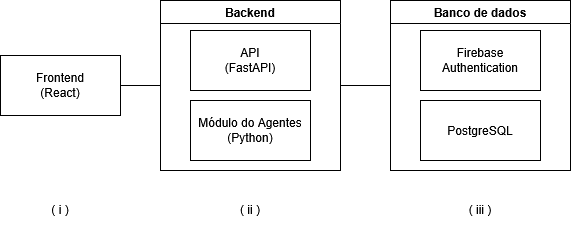
\includegraphics[width=0.6\textwidth]{Diagrama Arquitetura.png}
    \caption{Diagrama da arquitetura do sistema.}
    \label{fig:diagrama-sistema}
\end{figure}

\subsection{Agentes}

A plataforma Wumpus Verse disponibiliza três tipos de agentes com diferentes estratégias de decisão, todos projetados para maximizar a pontuação final, seja coletando o ouro, eliminando o Wumpus ou retornando à saída. A implementação desses agentes permite que os usuários comparem diferentes abordagens para o mesmo problema, facilitando a compreensão das vantagens e limitações de cada estratégia.

O \textbf{Agente Reativo Aleatório} implementa uma abordagem simples baseada em regras. A cada passo, o agente recebe as percepções da sala atual. Se detecta ouro, o agente o coleta imediatamente. Se detecta fedor, existe uma chance de 10\% de o agente atirar ou mover-se em uma direção aleatória. Este agente ignora completamente a percepção de brisa, o que o torna vulnerável a cair em poços, mas serve como um baseline para comparação com estratégias mais sofisticadas.

O \textbf{Agente Baseado em Modelo} mantém um estado interno, ou crença, que é atualizado continuamente com base nas percepções recebidas. Salas consideradas seguras são exploradas, enquanto salas com indícios de perigo são evitadas. Este agente utiliza o algoritmo A* para planejar rotas ótimas entre sua posição atual e os destinos desejados. O agente pode ser configurado com quatro perfis de comportamento distintos, que determinam sua estratégia de priorização:

\begin{itemize}
    \item \textbf{Perfil Assassino:} prioriza a localização e eliminação do Wumpus, mesmo que isso implique assumir riscos maiores.
    \item \textbf{Perfil Garimpeiro}: prioriza a coleta do ouro como objetivo principal, evitando confrontos desnecessários.
    \item \textbf{Perfil Explorador}: continua explorando o ambiente mesmo após cumprir seu objetivo inicial, buscando mapear completamente o cenário.
    \item \textbf{Perfil Corajoso}: está disposto a arriscar entrar em salas consideradas perigosas, confiando em sua capacidade de reagir a imprevistos.
\end{itemize}

O \textbf{Agente Evolutivo} emprega um algoritmo genético para otimizar uma sequência de ações (cromossomo), permitindo ao usuário configurar parâmetros populacionais, taxas genéticas e uma função fitness personalizada, combinação linear de passos, coleta de ouro e sobrevivência. A cada geração, os indivíduos são executados no ambiente, e os melhores são selecionados, recombinados e mutados; ao final, o melhor cromossomo define a política de ação do agente.

\subsection{Armazenamento e Backend}

O backend da plataforma Wumpus Verse é responsável por expor a API REST e gerenciar a persistência dos dados, assegurando que todas as informações geradas pelos usuários sejam armazenadas de forma segura e consistente. Para isso, sua arquitetura integra três aspectos fundamentais: a estrutura da API, a integração direta com os agentes e os mecanismos de persistência.

Desenvolvida em Python com o framework FastAPI, a API disponibiliza endpoints que cobrem todas as funcionalidades da plataforma. Os principais endpoints estão listados na Tabela~\ref{tab:endpoints-api}, que apresenta as rotas, métodos HTTP e descrições das operações disponíveis. A comunicação entre cliente e servidor utiliza JSON como formato de dados, e a maioria das requisições é autenticada via token JWT integrado ao Firebase Authentication, garantindo que apenas usuários autorizados possam acessar e modificar seus dados.

\begin{table}[ht]
    \centering
    \small
    \begin{tabular}{|p{5.5cm}|p{2cm}|p{6.5cm}|}
        \hline
        \underline{\textbf{Rota}} & \underline{\textbf{Método}} & \underline{\textbf{Descrição}} \\
        \hline
        \texttt{/environment/list-user}, \texttt{/environment/user} & GET, POST & Lista ou cria ambientes do usuário \\
        \hline
        \texttt{/environment/execution} & POST & Executa um agente em um ambiente (recebe IDs) \\
        \hline
        \texttt{/auth/register}, \texttt{/auth/login} & POST & Registro/login, retorna token JWT \\
        \hline
        \texttt{/agents/user}, \texttt{/agents/agents} & POST, GET & Cria ou lista agentes personalizado \\
        \hline
        \texttt{/execution/user}, \texttt{/execution/list-user} & POST, GET & Salva ou lista execuções \\
        \hline
        \texttt{/execution/statics} & POST & Analisa agentes em um ambiente (estatísticas) \\
        \hline
    \end{tabular}
    \caption{Endpoints da API para gerenciamento de ambientes, agentes e execuções.}
    \label{tab:endpoints-api}
\end{table}

Complementando a estrutura da API, a integração com os agentes foi projetada para otimizar o desempenho e a confiabilidade do sistema. Como os agentes também são implementados em Python, o backend os importa diretamente como módulos, eliminando a sobrecarga e a complexidade da comunicação entre linguagens diferentes. A simulação ocorre em um ambiente controlado (classe \texttt{Environment}), que recebe o agente e o grid, executa as ações passo a passo e coleta métricas como número de passos, ouro coletado, Wumpus morto e sobrevivência. Ao final da simulação, o sistema calcula a pontuação final do agente de acordo com as regras estabelecidas. Esse desenho permite a reciclagem de código entre a API e os agentes, reduzindo significativamente a complexidade e os possíveis pontos de falha.

Por fim, no que tange à persistência de dados, a plataforma adota dois sistemas de armazenamento complementares para gerenciar diferentes aspectos das informações. O \textbf{Firebase Authentication} é responsável pelo gerenciamento de cadastro, login e redefinição de senhas de usuários, fornecendo uma infraestrutura pronta e segura que elimina a necessidade de implementar esses mecanismos do zero. O \textbf{PostgreSQL}, por sua vez, é utilizado para armazenar os dados específicos da aplicação, incluindo ambientes (grid, posições), agentes (parâmetros, tipo, função fitness) e execuções (histórico, ouros coletados, Wumpus mortos, pontuação final). A escolha do PostgreSQL garante consistência transacional e integridade referencial, características essenciais para um sistema que lida com dados complexos e inter-relacionados. Dessa forma, a combinação dessas duas ferramentas proporciona uma base robusta e escalável para todas as operações de gerenciamento de usuários e experimentos realizados na plataforma.

\subsection{Frontend}

frontend da plataforma foi desenvolvido utilizando a biblioteca JavaScript React, permitindo a construção de uma interface web dinâmica e responsiva. A arquitetura da interface foi organizada em diferentes módulos, cada um responsável por uma etapa do fluxo de utilização do sistema, desde o acesso inicial até a execução e análise dos experimentos. Esta seção descreve os principais módulos da interface, relacionando cada funcionalidade aos requisitos funcionais estabelecidos na Seção~\ref{sec:req-arq-tec}.

A \textbf{tela de apresentação} constitui a página inicial da plataforma, fornecendo acesso às principais funcionalidades disponíveis, atendendo ao requisito de disponibilidade e acesso intuitivo ao sistema. Complementarmente, a seção \textbf{Saiba Mais} reúne informações sobre o projeto, sua motivação, a equipe de desenvolvimento e uma breve contextualização sobre o problema do Mundo do Wumpus.

O sistema possui um módulo de \textbf{autenticação} composto pelas telas de login e registro, responsáveis pelo gerenciamento do acesso dos usuários. O cadastro inclui verificação de e-mail, e apenas usuários autenticados podem acessar as funcionalidades de gerenciamento e execução de experimentos. Este módulo atende indiretamente aos requisitos de persistência (RF04) ao garantir que os dados sejam associados a usuários específicos.

Para a criação e administração dos cenários, a plataforma disponibiliza as telas \textbf{Mundos} e \textbf{Editor de Mundos}, atendendo ao requisito RF01 (Ambientes Personalizados). A primeira apresenta a lista de ambientes previamente criados pelo usuário, permitindo sua visualização, edição, exclusão, importação e exportação. O editor, por sua vez, possibilita a construção de mundos bidimensionais personalizados, nos quais podem ser posicionadas as entidades do jogo, como Wumpus, poços e ouro. Embora os cenários possam assumir diferentes formatos, sua estrutura é baseada em uma malha de salas quadradas interconectadas. A Figura~\ref{fig:telas-exemplos} apresenta exemplos dessas interfaces.

\begin{figure}[ht]
    \centering
    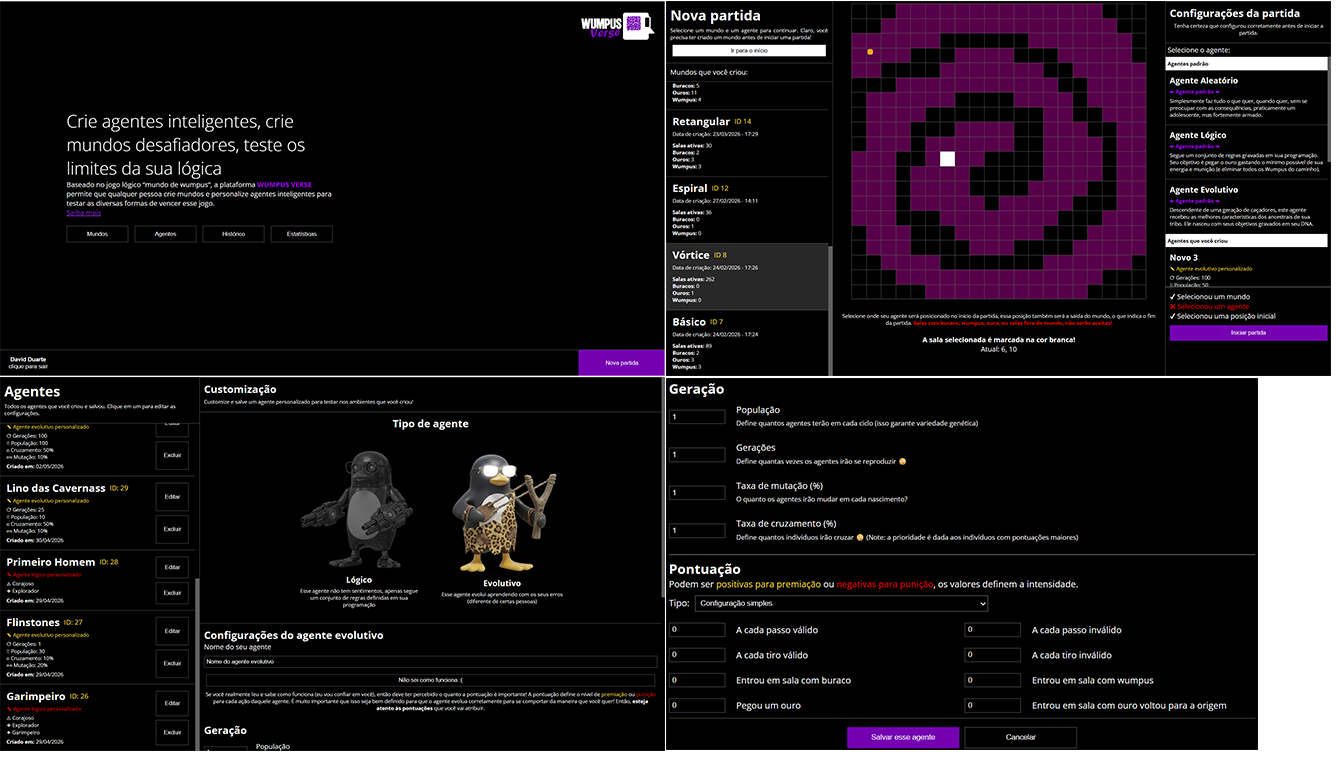
\includegraphics[width=0.6\textwidth]{telas-plataforma.png}
    \caption{Exemplo de telas da plataforma.}
    \label{fig:telas-exemplos}
\end{figure}

A tela \textbf{Agentes} permite criar e editar agentes lógicos e evolutivos (RF02). Para agentes lógicos, o usuário seleciona perfis de comportamento (assassino, garimpeiro, explorador, corajoso); para evolutivos, define parâmetros genéticos e função fitness personalizada, podendo experimentar combinações e observar os efeitos no comportamento.

As telas \textbf{Histórico} e \textbf{Estatísticas} (RF04 e RF05) gerenciam os resultados experimentais, permitindo recuperar execuções salvas e comparar agentes por métricas como pontuação média, passos e disparos. Para iniciar uma simulação, a tela \textbf{Nova Partida} (RF03) define o mundo, o agente e a posição inicial; na tela \textbf{Execução}, o trajeto do agente é reproduzido graficamente a partir do roteiro gerado pelo backend, com controles para navegação, repetição, ajuste de parâmetros e visualização das ações (Figura~\ref{fig:tela-execucao}).

\begin{figure}[ht]
    \centering
    
\includegraphics[width=0.6\textwidth]{tela-execução.png}
    \caption{Interface de execução da plataforma durante uma simulação.}
    \label{fig:tela-execucao}
\end{figure}

Além disso, o usuário pode armazenar a execução em sua conta para futuras análises, bem como exportar ou importar partidas por meio de arquivos, atendendo ao requisito RF06 (Exportação). A funcionalidade de exportação permite que os dados sejam salvos em formato JSON, enquanto a importação possibilita a reconstrução de ambientes e execuções previamente exportados.

Conforme mencionado anteriormente, a plataforma foi desenvolvida seguindo princípios de responsividade, permitindo seu acesso também por meio de dispositivos móveis. Entretanto, determinadas funcionalidades, como a criação e edição de mundos, permanecem disponíveis apenas em ambientes com teclado e mouse, uma vez que a definição da estrutura do cenário depende de interações de precisão baseadas no uso simultâneo do cursor e de comandos do teclado. Dessa forma, a adaptação para dispositivos móveis prioriza a consulta e a execução de experimentos, preservando a usabilidade das funcionalidades que demandam maior nível de interação. A Figura~\ref{fig:tela-mobile} apresenta a interface da plataforma em um dispositivo móvel, evidenciando a adaptação do layout para telas de menor dimensão.

\begin{figure}[ht]
    \centering
    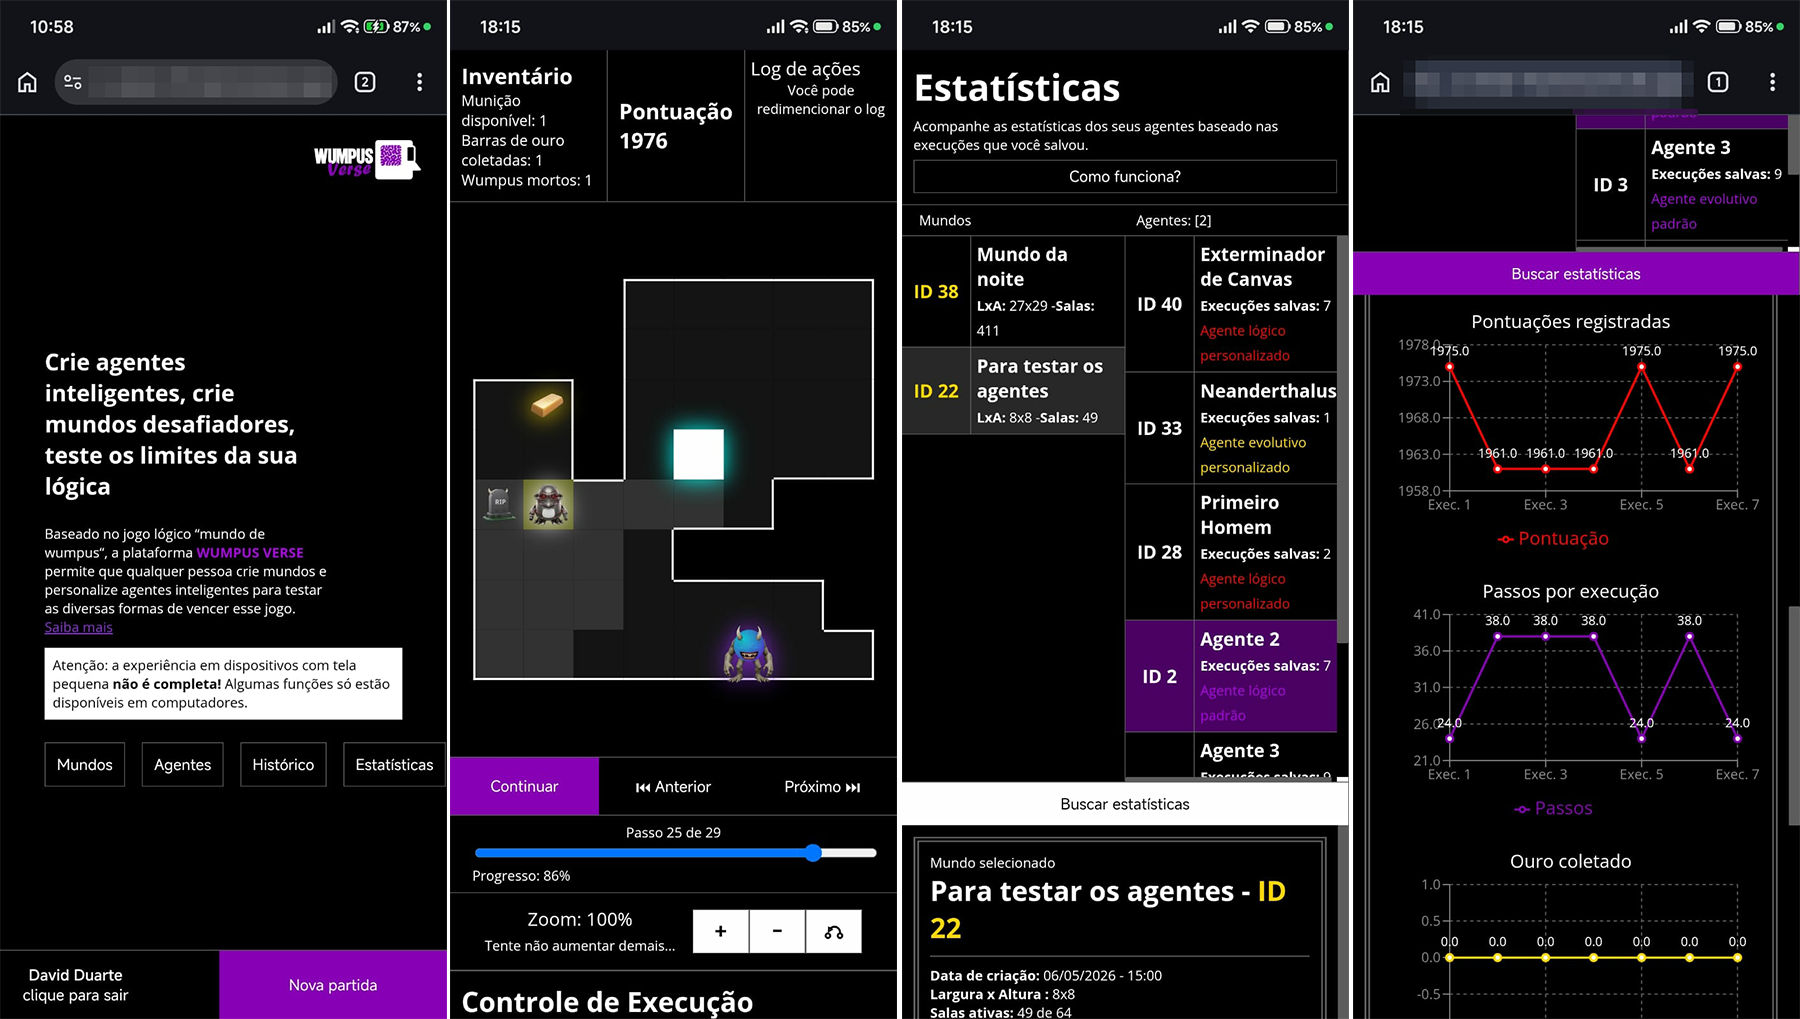
\includegraphics[width=0.5\textwidth]{telas-mobile.png}
    \caption{Interface responsiva da plataforma em dispositivo
móvel.}
    \label{fig:tela-mobile}
\end{figure}

\section{Análise Experimental}

A avaliação experimental da plataforma Wumpus Verse foi conduzida com o propósito de verificar o correto funcionamento de suas principais funcionalidades e a integração entre os módulos que compõem o sistema. Para isso, foram executados testes funcionais baseados em cenários representativos das ações que um usuário realiza durante a utilização da plataforma, abrangendo desde o cadastro e a autenticação até a criação de mundos e agentes, a execução de simulações, o armazenamento de resultados e as operações de importação e exportação de cenários. Dessa forma, buscou‑se assegurar que o comportamento observado estivesse em conformidade com os requisitos definidos para o protótipo.

\subsection{Objetivo da Validação}

A validação teve como objetivo principal verificar o funcionamento das funcionalidades disponibilizadas pela plataforma, avaliando sua capacidade de executar corretamente as operações previstas e de integrar os diferentes módulos do sistema. Além disso, procurou‑se identificar eventuais limitações ou aspectos que ainda necessitassem de ajustes, garantindo que os usuários pudessem realizar as tarefas essenciais do fluxo de utilização sem a ocorrência de falhas críticas. Para tanto, foram considerados aspectos relacionados à autenticação, ao gerenciamento de mundos, à criação e configuração de agentes, à execução e ao armazenamento de simulações, à geração de estatísticas e à manipulação de dados por meio dos recursos de importação e exportação.

\subsection{Metodologia de Testes}

A validação da plataforma foi realizada por meio de testes funcionais manuais baseados em cenários de uso. Essa abordagem foi adotada por ser adequada para avaliar o comportamento das funcionalidades implementadas em uma aplicação que ainda se encontra em fase de prototipação, permitindo verificar diretamente os resultados obtidos a partir das ações executadas pelo usuário. Para cada cenário de teste, foi definida uma funcionalidade alvo, um critério de sucesso correspondente ao comportamento esperado e o resultado observado durante a execução. Os cenários foram elaborados de modo a contemplar as principais etapas de utilização da plataforma, abrangendo o gerenciamento de usuários, ambientes e agentes, bem como a execução, a consulta e a manipulação dos resultados das simulações.

A Tabela 2 apresenta os cenários utilizados durante a validação, juntamente com os respectivos critérios de sucesso e resultados observados.

\begin{table}[ht]
    \centering
    \caption{Apresenta os cenários de teste.}
    \label{tab:cenario-testes}
    \small
    \begin{tabular}{|p{1cm}|p{4.5cm}|p{6.5cm}|p{2cm}|}
        \hline
        \textbf{ID} & \textbf{Funcionalidade} & \textbf{Critério de Sucesso}  & \textbf{Resultado} \\
        \hline
        CT01 & Cadastro de usuário & Usuário cadastrado com sucesso & Funcional \\
        \hline
        CT02 & Login na plataforma & Autenticação realizada corretamente & Funcional \\
        \hline
        CT03 & Criação de mundo & Mundo criado e armazenado sem erros & Funcional \\
        \hline
        CT04 & Criação de agentes & Agente criado e salvo corretamente & Funcional \\
        \hline
        CT05 & Funcionamento dos agentes & Agente realiza ações coerentes no ambiente & Ajustes \hbox{Planejados} \\
        \hline
        CT06 & Execução de simulação & Simulação executada e resultados apresentados ao usuário & Ajustes \hbox{Planejados} \\
        \hline
        CT07 & Visualização do histórico & Execuções exibidas corretamente & Funcional \\
        \hline
        CT08 & Geração de estatísticas & Métricas apresentadas corretamente & Ajustes \hbox{Planejados} \\
        \hline
        CT09 & Salvamentos de resultados & Resultados armazenados com sucesso & Funcional \\
        \hline
        CT10 & Exportação para JSON & Arquivo JSON gerado & Funcional \\
        \hline
        CT11 & Importação de mapas & Mapa carregado e reconstruído corretamente & Funcional \\
        \hline
    \end{tabular}
    \\{\small Fonte: Elaborado pelo autor.}
\end{table}

Conforme evidenciado na Tabela 2, as funcionalidades relacionadas ao gerenciamento de usuários, à criação de mundos e agentes, à visualização do histórico, ao armazenamento de resultados e às operações de importação e exportação apresentaram comportamento funcional durante os testes. Por outro lado, as funcionalidades associadas ao comportamento dos agentes, à execução das simulações e à geração de estatísticas foram classificadas como "ajustes planejados", indicando que esses componentes ainda demandam aprimoramentos no protótipo.

\subsection{Cenário Demonstrativo}

Para complementar a avaliação funcional, foi considerado um cenário demonstrativo que representa o fluxo completo de utilização da plataforma. Nesse cenário, o usuário inicia sua interação realizando o cadastro e a autenticação no sistema. Após o acesso, ele cria um mundo do Wumpus e configura um agente para atuar nesse ambiente, permitindo verificar a integração entre os recursos de gerenciamento de usuários, ambientes e agentes. Em seguida, o usuário executa uma simulação e acompanha o comportamento do agente durante sua interação com o mundo. Após a execução, são consultadas as estatísticas disponibilizadas pela plataforma para avaliar as informações produzidas durante a simulação. Os resultados obtidos são então armazenados no sistema e podem ser posteriormente recuperados por meio do histórico de execuções. Por fim, o cenário contempla a exportação dos dados do ambiente em formato JSON, seguida da importação do arquivo gerado, o que permite verificar se as informações exportadas podem ser utilizadas para reconstruir o mapa na plataforma. Dessa forma, o cenário demonstrativo reúne diferentes funcionalidades do sistema em um único fluxo, evidenciando a integração entre os módulos envolvidos.

\subsection{Discussão dos Resultados}

Os testes funcionais realizados demonstraram que a plataforma Wumpus Verse apresenta funcionamento adequado em suas principais funcionalidades de gerenciamento e persistência. Os recursos de cadastro e autenticação de usuários, criação de mundos e agentes, visualização do histórico, armazenamento de resultados e importação/exportação de cenários comportaram‑se conforme o esperado. A criação de agentes também se mostrou operacional, embora os mecanismos de personalização ainda estejam em processo de refinamento, uma vez que algumas opções de configuração necessitam de ajustes para oferecer maior flexibilidade e uma melhor experiência de utilização. Essa limitação está relacionada principalmente à necessidade de ampliar as possibilidades de configuração dos agentes disponibilizadas pela plataforma.

No que diz respeito à execução das simulações, o comportamento observado nos cenários avaliados foi considerado satisfatório, mas a tomada de decisão dos agentes e a integração com serviços externos ainda requerem aprimoramentos. Em particular, a utilização de uma API externa em sua versão gratuita pode introduzir limitações de desempenho e ocasionar eventuais inconsistências durante determinadas execuções. Outro aspecto identificado está relacionado ao módulo de estatísticas e análise dos resultados: atualmente, a plataforma disponibiliza informações básicas sobre as execuções realizadas, mas a quantidade de métricas ainda pode ser ampliada para proporcionar uma análise mais detalhada do desempenho dos agentes em diferentes cenários.

De modo geral, os resultados obtidos indicam que o protótipo atende às principais funcionalidades propostas, especialmente aquelas voltadas ao gerenciamento dos ambientes, agentes e resultados experimentais. Ao mesmo tempo, os testes permitiram identificar funcionalidades que ainda necessitam de evolução, fornecendo uma base sólida para o direcionamento dos trabalhos futuros. Entre os principais aprimoramentos planejados, destacam‑se a ampliação das opções de personalização dos agentes, o aumento da robustez da integração com serviços externos, o aperfeiçoamento dos mecanismos de tomada de decisão e a disponibilização de métricas mais detalhadas para a análise de desempenho no ambiente do Mundo do Wumpus.





\section{Conclusão}

Este trabalho apresentou o Wumpus Verse, um protótipo de plataforma web desenvolvido para apoiar a criação, execução e avaliação de agentes inteligentes no ambiente do Mundo do Wumpus. A proposta surgiu da necessidade de disponibilizar uma ferramenta acessível e integrada que permitisse a experimentação com agentes inteligentes sem exigir dos usuários conhecimentos avançados de programação ou configuração de ambientes de teste.

A plataforma foi projetada para oferecer recursos que abrangem todo o ciclo de experimentação, incluindo a criação de mundos personalizados, a configuração de diferentes tipos de agentes, a execução de simulações, o armazenamento de resultados e a geração de estatísticas de desempenho. Além disso, sua implementação em ambiente web amplia a acessibilidade da ferramenta, permitindo sua utilização para a realização de experimentação em lote e padronização de métricas.

Os testes realizados demonstraram o funcionamento adequado das principais funcionalidades do sistema, evidenciando a integração entre os módulos desenvolvidos e a capacidade da plataforma de fornecer um ambiente consistente para a realização de experimentos envolvendo agentes inteligentes.

Como perspectivas futuras, pretende-se ampliar as funcionalidades da plataforma de modo a torná-la ainda mais flexível e personalizável. Uma das principais evoluções planejadas está relacionada ao modelo de construção dos ambientes. Atualmente, embora os mundos possam assumir diferentes formatos por meio da adição de salas em posições arbitrárias, sua estrutura ainda permanece limitada a uma malha bidimensional. Como extensão, pretende-se permitir a criação de conexões manuais entre salas, de forma semelhante a diagramas ou grafos, possibilitando a construção de ambientes com topologias mais complexas e menos restritas ao modelo tradicional do Mundo de Wumpus.

Também estão previstas melhorias nos mecanismos de execução das simulações, oferecendo maior controle sobre parâmetros experimentais e ampliando as opções de configuração disponíveis aos usuários. Dessa forma, espera-se proporcionar maior flexibilidade para a realização de diferentes tipos de experimentos e análises.

Outra funcionalidade de interesse é o suporte a múltiplos agentes atuando simultaneamente em um mesmo ambiente. Essa extensão permitirá a investigação de cenários cooperativos e competitivos, ampliando significativamente as possibilidades de estudo e avaliação de estratégias de tomada de decisão.

Por fim, prevê-se a incorporação de recursos voltados à interação entre usuários, como compartilhamento de mundos e agentes, sistemas de classificação e mecanismos de colaboração.

Com essas evoluções, espera-se consolidar o Wumpus Verse como uma plataforma cada vez mais completa e acessível para atividades de ensino, pesquisa e experimentação envolvendo agentes inteligentes.

\bibliographystyle{tcc}
\bibliography{tcc-template}

\end{document}
